\chapter{Priority Queues}
\label{ch:pq}

\newcommand{\lecnum}{17}
%\newcommand{\lectitle}{Priority Queues}
\newcommand{\lecturer}{Frank Pfenning, Rob Simmons}

\chapterTAGS{array, complexity, ds-invariant, interface, pq, stack}
\maketitle

\begin{preamble}
\noindent
In this lecture we will look at \emph{priority queues} as an abstract type and
discuss several possible implementations.  We then pick the representation as
\emph{heaps} and start to work towards an implementation (which we will
complete in the next lecture).  Heaps have the structure of binary trees, a
very common structure since a (balanced) binary tree with $n$ elements has
height $O(\log n)$.  During the presentation of algorithms on heaps we will
also come across the phenomenon that invariants must be temporarily violated
and then restored.  We will study this in more depth in the next lecture.
From the programming point of view, we will see a cool way to implement binary
trees in arrays which, alas, does not work very often.
\end{preamble}

\begin{gram}[Learning Goals]
This maps as follows to our learning goals:
\begin{description}
\item[Computational Thinking: ]%
  We focus on the trade-offs of various representations for a given data
  structure, and dip our toes in the idea of temporarily violating
  invariants.

\item[Algorithms and Data Structures: ]%
  We introduce priority queues, a common data structure for prioritized
  task lists, and heaps, an efficient way to implement them.

\item[Programming: ]%
  For once, we won't be doing any programming in this lecture!
\end{description}
\end{gram}

\section{Priority Queues}
\label{sec:pq:intro}
\TAGS{interface, pq, stack}

A priority queue is like a queue, a stack, or an unbounded array: there's an
add function (\lstinline'enq', \lstinline'push', \lstinline'uba_add') and a
delete function (\lstinline'deq', \lstinline'pop', \lstinline'uba_rem').
Stacks and queues can be generally referred to as \emph{worklists}. A priority
queue will be a new kind of worklist.  We think of each element as a task: we
put all the work we need to do on the worklist (with
\lstinline'enq'/\lstinline'push'/\lstinline'add'), and then consult the
worklist to find out what work we should do next (with
\lstinline'deq'/\lstinline'pop'/\lstinline'rem').

Queues and stacks have a \emph{fixed} way of deciding which element
gets removed: queues always remove the element that was added first
(FIFO), and stacks always remove the element that was added most
recently (LIFO). This makes the client interface for generic stacks
and queues very easy: the queue or stack doesn't need to know anything
about the generic type \lstinline'elem'. The library doesn't even need to
know if \lstinline'elem' is a pointer. (Of course, as clients, we'll
probably want \lstinline'elem' to be defined as the generic type
\lstinline'void*'.)

For example, here's again the interface for stacks:
\begin{lstlisting}[language={[C0]C}]
/* Client interface for stacks */
// typedef _______ elem;

/* Library interface for stacks */
// typedef ______* stack_t;

bool stack_empty(stack_t S)
  /*@requires S != NULL; @*/ ;

stack_t stack_new()
  /*@ensures \result != NULL; @*/ ;

void push(stack_t S, elem x)
  /*@requires S != NULL; @*/ ;

elem pop(stack_t S)
  /*@requires S != NULL && !stack_empty(S); @*/ ;
\end{lstlisting}
Rather than fixing, once and for all, the definition of what elements will get
returned first, priority queues allow the client to decide in what order
elements will get removed. The client has to explain how to give every element
a \emph{priority}, and the priority queue ensures that whichever element has
the \emph{highest priority} will get returned first. For example, in an
operating system the runnable processes might be stored in a priority queue,
where certain system processes are given a higher priority than user
processes.  Similarly, in a network router packets may be routed according to
some assigned priorities.

\clearpage
To implement the library of priority queues, we need the user
to give us a function \lstinline'has_higher_priority(x,y)' that returns true
only when \lstinline'x' has strictly higher priority than \lstinline'y'.

\begin{lstlisting}[language={[C0]C}]
/* Client-side interface for priority queues */
// typedef _______ elem;

typedef bool has_higher_priority_fn(elem e1, elem e2);
\end{lstlisting}

Once we've defined the client interface for priority queues, the interface is
very similar to the stacks and queues we've seen before: \lstinline'pq_new'
creates a new priority queue, \lstinline'pq_empty' checks whether any elements
exist, and \lstinline'pq_add' and \lstinline'pq_rem' add and remove elements,
respectively. We also add a function \lstinline'pq_peek' which returns the
element that should be removed next without actually removing it. For stacks,
this operation can be implemented on the client-side in constant time, but
that is not the case for queues and may not be the case for priority queues.


%%  represented by an integer.  We always
%% remove an element with the highest priority, which is given by the
%% \emph{minimal} integer priority assigned.  Priority queues often have
%% a fixed size.


%% Here is an abstract interface to a (bounded) priority queue.  Our
%% implementation uses a data structure call a \emph{heap} which we
%% discuss shortly.
\begin{lstlisting}[language={[C0]C}]
/* Library-side interface */
// typedef ______* pq_t;

bool pq_empty(pq_t P)
  /*@requires P != NULL; @*/ ;

pq_t pq_new(has_higher_priority_fn* prior)
  /*@requires prior != NULL; @*/
  /*@ensures \result != NULL; @*/
  /*@ensures pq_empty(\result); @*/ ;

void pq_add(pq_t P, elem x)
  /*@requires P != NULL; @*/ ;

elem pq_rem(pq_t P)
  /*@requires P != NULL && !pq_empty(P); @*/ ;

elem pq_peek(pq_ P)
  /*@requires P != NULL && !pq_empty(P); @*/ ;
\end{lstlisting}

In this lecture, we will actually use heaps to implement
\emph{bounded} priority queues. When we create a bounded worklist, we
pass a strictly positive maximum capacity to the function that creates
a new worklist (\lstinline'pq_new'). We also add a new function that
checks whether a worklist is at maximum capacity
(\lstinline'pq_full'). Finally, it is a precondition to
\lstinline'pq_add' that the priority queue must not be full.  Bounding
the size of a worklist may be desirable to prevent so-called
\emph{denial-of-service attacks} where a system is essentially
disabled by flooding its task store.  This can happen accidentally or
on purpose by a malicious attacker.  To accommodate this, we make the
following addition and changes to the above interface:
\begin{lstlisting}[language={[C0]C}]
/* Library-side interface -- heap implementation */
// ...

bool pq_full(pq_t P)
  /*@requires P != NULL; @*/ ;

pq_t pq_new(int capacity, has_higher_priority_fn* prior) // NEW argument
  /*@requires capacity > 0 && prior != NULL; @*/ // NEW check
  /*@ensures \result != NULL; @*/
  /*@ensures pq_empty(\result); @*/ ;

void pq_add(pq_t P, elem x)
  /*@requires P != NULL && !pq_full(P); @*/ ; // NEW call

\end{lstlisting}


%% On the client side we must have a function that extracts the priority
%% of an element, since the library cannot know in general what this
%% priority would be.  We could just use integers directly, having each
%% element return an integer priority. Alternatively, we could extract
%% abstract keys, and compare the priority of those abstract keys. We
%% will instead use a third solution: we will define an abstract notion
%% of comparing the priorities of two elements,
%% \lstinline'has_higher_priority(e1,e2)', that returns true when \lstinline'e1' is
%% strictly higher priority than \lstinline'e2'.


\section{Some Implementations}
\label{sec:pq:strawmen}
\TAGS{complexity, pq}

Before we come to heaps, it is worth considering different
implementation choices for bounded priority queues and consider the
complexity of various operations.

The first idea is to use an unordered array where the length of the
array is the maximum capacity of the priority queue, along with a
current size  $n$. Inserting into such an array is a constant-time
operation, since we only have to insert it at $n$ and increment $n$.
However, finding the highest-priority element (\lstinline'pq_peek') will
take $O(n)$, since we have to scan the whole portion of the array
that's in use.  Consequently, removing the highest-priority element
also takes $O(n)$: first we find the highest-priority element, then we
swap it with the last element in the array, then we decrement $n$.

A second idea is to keep the array sorted.  In this case, inserting an element
is $O(n)$.  We can quickly (in $O(\log n)$ steps) find the place $i$ where it
belongs using binary search, but then we need to shift elements to make room
for the insertion.  This takes $O(n)$ copy operations. Finding the
highest-priority element is definitely $O(1)$, and if we arrange the array so
that the highest-priority elements are at the end, deletion is also $O(1)$.

If we instead keep the elements sorted in an AVL tree, the AVL height
invariant ensures that insertion becomes a $O(\log n)$ operation. We
haven't considered deletion from AVL trees, though it can be done in
logarithmic time.

The heap structure we present today also gives logarithmic time for
adding an element and removing the element of highest priority. Heaps
are also more efficient, both in terms of time and space, than using
balanced binary search trees, though only by a constant factor.

In summary:
$$
\begin{array}{lccc}
                          & \mathtt{pq\_add}& \mathtt{pq\_rem}& \mathtt{pq\_peek}
\\ \text{unordered array} & O(1)              & O(n)              & O(n)
\\ \text{ordered array}   & O(n)              & O(1)              & O(1)
\\ \text{AVL tree}        & O(\log n)         & O(\log n)         & O(\log n)
\\ \text{heap}            & O(\log n)         & O(\log n)         & O(1)
\end{array}
$$

\section{The Min-heap Ordering Invariant}
\label{sec:pq:minheap_ordering}
\TAGS{ds-invariant, pq}

A \emph{min-heap} is a binary tree structure, but it is a very
different binary tree than a binary search tree.

The min-heaps we are considering now can be used as priority queues of
\underline{integers}, where \emph{smaller} integers are treated as having
\emph{higher priority}. (The alternative is a \emph{max-heap},
where \emph{larger} integers are treated as having higher priority.)
Therefore, while we focus our discussion on heaps, we will talk about
``removing the minimal element'' rather than ``removing the element
with the highest priority.''

Typically, when using a priority queue, we expect the number of
inserts and deletes to roughly balance.  Then neither the unordered
nor the ordered array provide a good data structure since a sequence
of $n$ inserts and deletes will have worst-case complexity $O(n^2)$.
A heap uses binary trees to do something in between ordered arrays
(where it is fast to remove) and unordered arrays (where it is fast to
add).

A min-heap is a binary tree where the invariant guarantees that
the minimal element is at the root of the tree.  For this to be the
case we just require that the key of a node be less than or equal to the
keys of its children.  Alternatively, we could say that each node
except the root is greater than or equal to its parent.
\begin{description}
\item[Min-heap ordering invariant (alternative 1): ] %
  The key of each node in the tree is less than or equal to all of its
  children's keys.
\item[Min-heap ordering invariant (alternative 2): ]%
  The key of each node in the tree except for the root is greater than or
  equal to its parent's key.
\end{description}
These two characterizations are equivalent.  Sometimes it turns out to
be convenient to think of it one way, sometimes the other.  Either of
them implies that the minimal element in the heap is a the root, due
to the transitivity of the ordering.  Therefore, we can expect that we
can find the minimal element in $O(1)$ time.


\section{The Heap Shape Invariant}
\label{sec:pq:heap_shape}
\TAGS{ds-invariant, pq}

We'll simultaneously give heaps a second invariant:
we fill the tree level by level, from left to right.  This
means the shape of the tree is completely determined by the number
of elements in it.  Here are the shapes of heaps with 1 through 7
nodes:
\begin{center}
  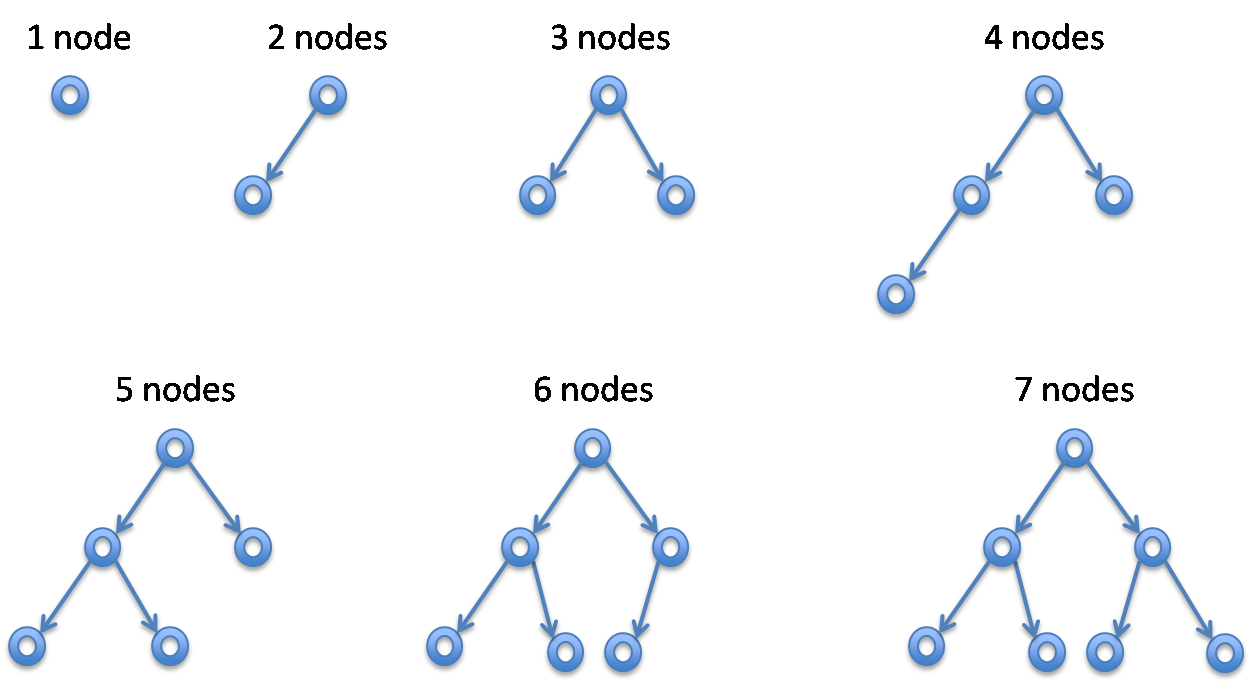
\includegraphics[width=0.9\textwidth]{img/heap1.png}
\end{center}
We call this latter invariant the \emph{heap shape invariant}.  A tree
that has the heap shape invariant is almost perfectly balanced.

The heap shape invariant would not be a useful invariant for a binary
search tree, because it is too costly to do insertion in a binary
search tree while maintaining both the binary search tree ordering
invariant and the heap shape invariant.  As we will see, we can do
addition to heaps and removal from heaps quite efficiently while maintaining
both the heap shape invariant and the heap ordering invariant.

\section{Adding to a Heap}
\label{sec:pq:inserting}
\TAGS{ds-invariant, pq}

When we add a new integer to a min-heap, we already know (by the shape
invariant) where a new node has to go.  However, we cannot simply put
the new data element there, because it might violate the ordering
invariant.  We do it anyway and then work to restore the invariant.
We will talk more about temporarily violating a data structure
invariant in the next lecture, as we develop code.  Let's consider an
example.  On the left is the heap before insertion of data with key 1;
on the right after, but before we have restored the invariant.
\begin{center}
  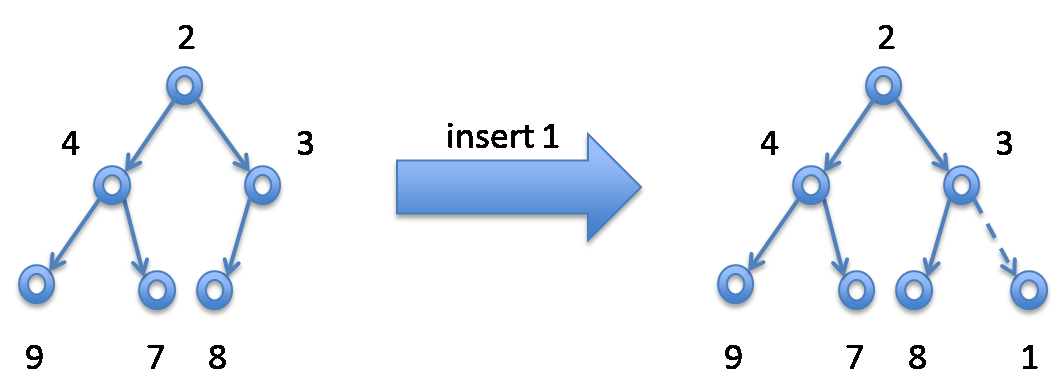
\includegraphics[width=0.9\textwidth]{img/insert1.png}
\end{center}
The dashed line indicates where the ordering invariant might
be violated.  And, indeed, $3 > 1$.

We can fix the invariant at the dashed edge by swapping the two
nodes.  The result is shown on the right.
\begin{center}
  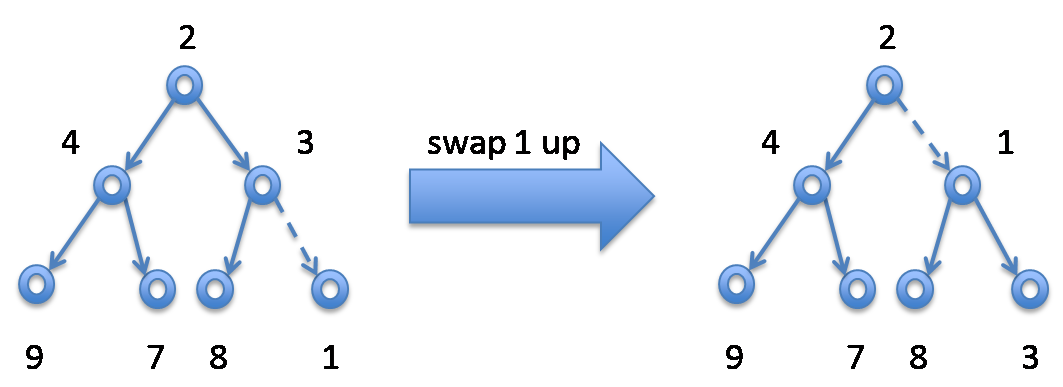
\includegraphics[width=0.9\textwidth]{img/swap1up-a.png}
\end{center}
The link from the node with key $1$ to the node with key $8$ will
always satisfy the invariant, because we have replaced the previous
key $3$ with a smaller key ($1$).  But the invariant might now be
violated going up the tree to the root.  And, indeed $2 > 1$.

We repeat the operation, swapping $1$ with $2$.
\begin{center}
  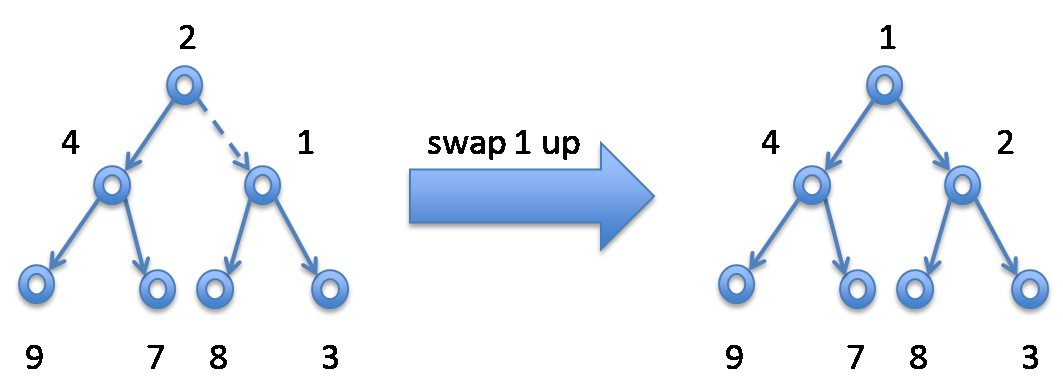
\includegraphics[width=0.9\textwidth]{img/swap1up-b.png}
\end{center}
As before, the link between the root and its left child continues to
satisfy the invariant because we have replaced the key at the root with
a smaller one.  Furthermore, since the root node has no parent, we
have fully restored the ordering invariant.

In general, we swap a node with its parent if the parent has a
strictly greater key.  If not, or if we reach the root, we have
restored the ordering invariant.  The shape invariant was always
satisfied since we inserted the new node into the next open place in
the tree.

The operation that restores the ordering invariant is called \emph{sifting
  up}, since we take the new node and move it up the heap until the invariant
has been reestablished.  The complexity of this operation is $O(l)$, where $l$
is the number of levels in the tree.  For a tree of $n \geq 1$ nodes there are
$\log_2 n +1$ levels.  So the complexity of inserting a new node is $O(\log n)$,
as promised.

\section{Removing the Minimal Element}
\label{sec:pq:removing}
\TAGS{ds-invariant, pq}

To delete the minimal element from a min-heap we cannot simply delete
the root node where the minimal element is stored, because we would
not be left with a tree.  But by the shape invariant we know how the
post-deletion tree has to be shaped.  So we take the \emph{last}
element in the bottom-most level of the tree and move it to the root,
and delete that last node.
\begin{center}
  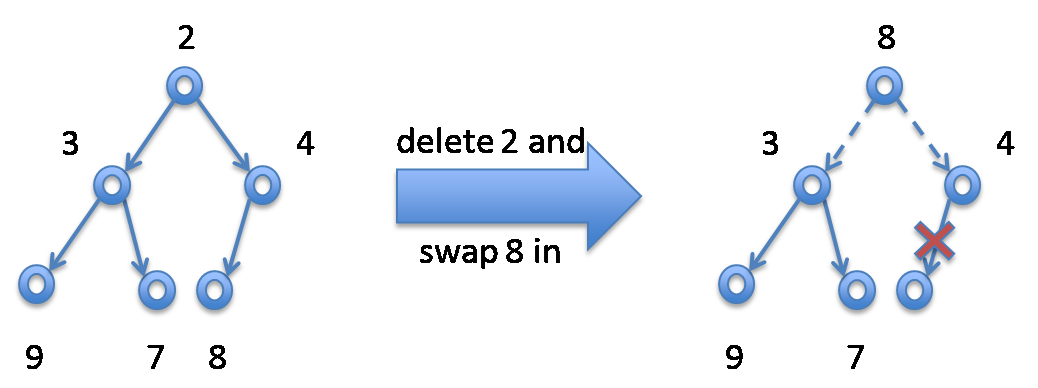
\includegraphics[width=0.9\textwidth]{img/delete2.png}
\end{center}
However, the node that is now at the root might have a strictly
greater key than one or both of its children, which would violate the
ordering invariant.

% \clearpage
If the ordering invariant in indeed violated, we swap the node
with the \emph{smaller} of its children.
\begin{center}
  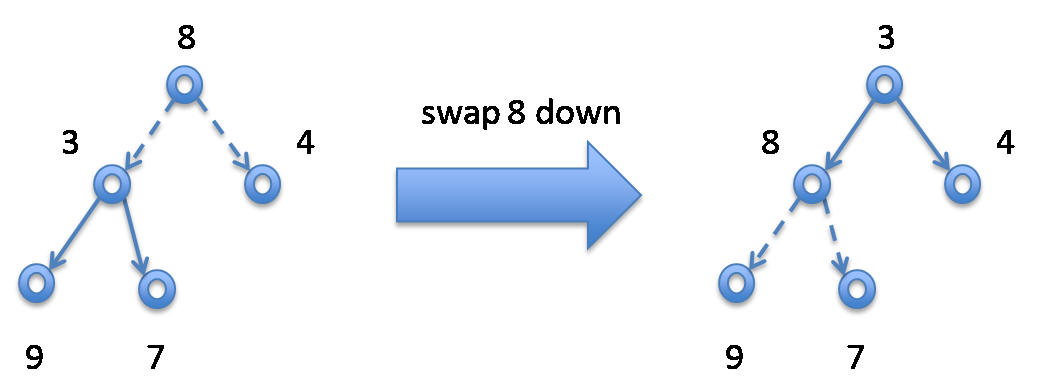
\includegraphics[width=0.9\textwidth]{img/swap8down-a.png}
\end{center}

This will reestablish the invariant at the root.  In general we see
this as follows.  Assume that before the swap the invariant is
violated, and the left child has a smaller key than the right one.  It
must also be smaller than the root, otherwise the ordering invariant
would hold.  Therefore, after we swap the root with its left child,
the root will be smaller than its left child.  It will also be smaller
than its right child, because the left was smaller than the right
before the swap.  When the right child is smaller than the left, the
argument is symmetric.

Unfortunately, we may not be done, because the invariant might now
be violated at the place where the old root ended up.  If not, we stop.
If yes, we compare the children as before and swap with the smaller
one.
\begin{center}
  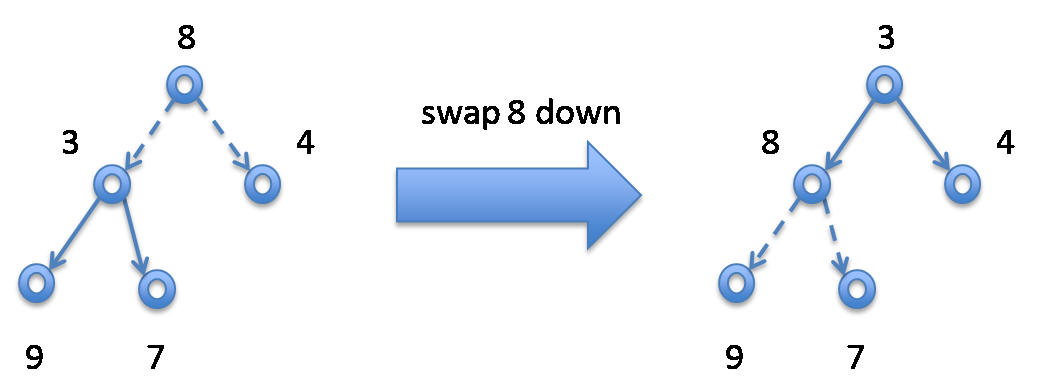
\includegraphics[width=0.9\textwidth]{img/swap8down-a.png}
\end{center}

We stop this downward movement of the new node if either the ordering
invariant is satisfied, or we reach a leaf.  In both cases we have fully
restored the ordering invariant.  This process of restoring the invariant is
called \emph{sifting down}, since we move a node down the tree.  As in the
case for insert, the number of operations is bounded by the number of levels
in the tree, which is $O(\log n)$ as promised.

\section{Representing Heaps as Arrays}
\label{sec:heap_impl}
\TAGS{array, ds-invariant, pq}

A first thought on how to represent a heap would be using structs with
pointers.  The sift-down operation follows the pointers from nodes to their
children, and the sift-up operation goes from children to their parents.  This
means all interior nodes require three pointers: one to each child and one to
the parent, the root requires two, and each leaf requires one. We'd also need
to keep track of the number of nodes in the tree.

While a pointer structure is not unreasonable, there is a more elegant
representation using arrays.  We use binary numbers as addresses of
tree nodes, numbering nodes level by level starting at the root, and
left to right on each level.  Assume a node has index $i$.  Then we
append a $0$ to the binary representation of $i$ to obtain the index
for the left child and a $1$ to obtain the index of the right child.
We start at the root with the number $1$.  If we tried to use $0$,
then the root and its left child would get the same address.  The node
number for a full three-level tree on the left in binary and on the
right in decimal.
\begin{center}
  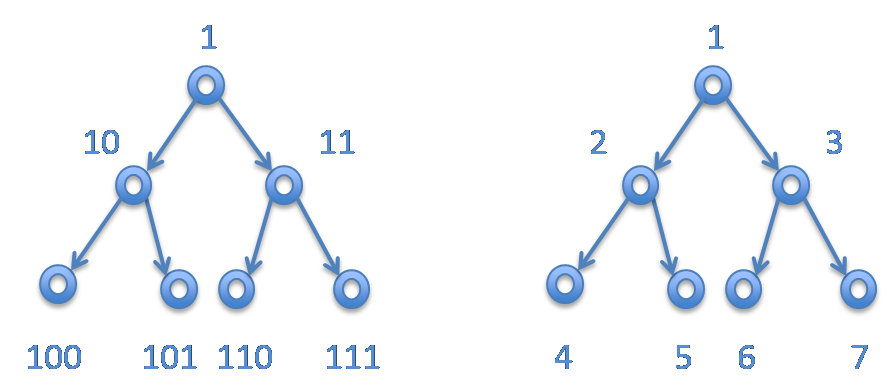
\includegraphics[width=0.8\textwidth]{img/heapcount.png}
\end{center}
Mapping this back to numeric operations, for a node at index $i$ we
obtain its left child as $2i$, its right child as $2i+1$, and its
parent as $i/2$.  Care must be taken, since any of these may be out of
bounds of the array.  A node may not have a right child, or neither
right nor left child, and the root does not have a parent.

In the next lecture we will write some code to implement heaps
and reason about its correctness.

\clearpage
\section{Exercises}
\label{sec:pq:exercises}

\begin{exercise}
  One of many options is using a sorted linked list instead of a
  sorted array to implement priority queues. What is the complexity of
  the priority queue operations on this representation? What are the
  advantages/disadvantages compared to an ordered array?
\end{exercise}

\begin{exercise}
  Consider implementing priority queues using an unordered list
  instead of an unordered array to implement priority queues. What is
  the complexity of the priority queue operations on this
  representation? What are the advantages/disadvantages compared to an
  unordered array?
\end{exercise}

% \clearpage
% \bibliographystyle{alpha}
% \bibliography{modal}

% \cleardoublepage
